\chapter{绪论}

\section{研究背景}
\indent
文化兴则国运兴,文化强则民族强。文化是国家的灵魂,民族的血液。2024年7月,党的二十届三中全会胜利完会,全会审议通过的《中共中央关于进一步全面深化改革、推进中国式现代化的决定》 ~\cite{xjptheory1} 中特别指出,要优化文化产品供给机制,激发全民族文化创新创造活力,这其中有两个着力点,就是强化创作导向、借力技术创新。为了更好更牢地以文化为重要支点推动经济高质量发展,不断实现文化与经济交融互动、融合发展,我们需要积极推进以文兴业、科技赋能,大力发展以“文化+创意”“文化+科技”为主要特征的文化创意产业,成为有效应对发展挑战、培育新的经济增长点的突破口~\cite{theory2} 。尽管文创领域发展一片良好,但现阶段还是存在一些问题:
\newline \indent
(1)文创产品的质量不够高,难以满足人们日益增长的审美需求。
\newline \indent
(2)文创开发的效率较低下,对于某一难以在短时间内产出多种相关的创作成果,难以在快速波动的市场中抓住商业机会。
\newline \indent
为了更好地聚焦于两个着力点,强化文化数字产品的创作能力,有效提升我国文化创作水平,我们可以利用风格迁移技术。风格迁移技术是一种强大的技术,通过往特定场景中引入风格化图像的风格特征并融合处理,创造出新的风格化的艺术场景。其中二维图像风格迁移可以用在广告、设计和媒体等领域,通过改变图像的外观和装饰,使其更加引人注目和独特。三维风格迁移是将一个场景的风格提取并且应用到另一个场景的三维模型上,可以为虚拟现实、游戏开发和电影制作等领域注入新动能,推动文化产业的创新创优,丰富人民的文化生活。
\newline \indent
经过多年的发展,风格迁移技术得到了长足进步,但是还是存在以下问题~\cite{jing2019neural}:
\newline \indent
(1)图像的风格纹理特征不够细致。现有的图像的任意风格迁移算法不能在生成无伪影的高质量图像的同时充分兼顾如颜色,笔触,色调,纹理等艺术特征,导致。现有的内容和风格特征之间对齐的方法还需要进一步完善,以保障更高质量的特征混合。同时现有的风格特征使用VGG~\cite{simonyan2014very}编码器进行提取,它更适合分类任务的特征处理,而在关注颜色,笔触、纹理等艺术特征方面还可以进一步优化。
\newline \indent
(2)3D场景风格迁移技术的性能权衡问题:现有的3D场景迁移模型多少在以下方面有一些不足:多视角一致性不够、对任意一个新的风格图片都需要重新进行风格化训练、训练推理速度较慢等、在面对更多的约束和挑战下,场景的风格化质量不佳等。有的模型结构过于复杂对设备要求较高,而且将它们应用到现实中充满各种物体的3D环境中存在较大不足。


% \begin{enumerate}
%     \item 删除根目录的 ``.latexmkrc'' 文件,否则编译失败且不报任何错误
%     \item 字体有版权所以本模板不能附带字体,请务必手动上传字体文件,并在各个专业模板下手动指定字体。
%         具体方法参照 GitHub 主页的说明。
% \end{enumerate}


\section{研究目标及内容}
近年来,随着经济科技的快速发展,人们对于文化艺术产品的要求也越来越高。艺术风格迁移作为一种通过将风格注入到内容载体中来创造视觉上有吸引力的图像的方法越来越受欢迎。但是现有的2D风格迁移方法无法在较好地考虑风格的颜色,笔触,色调,纹理等艺术特征地同时做到无伪影地风格迁移。与此同时,现有的3D场景风格迁移技术,均不同程度地存在多视角一致性不够、无法做到零样本迁移、对算力要求较高、训练推理速度较慢等。因此,本文的研究目标是针对设计一个新的2D图像任意风格迁移算法,并提出一个支持不同风格迁移方法的零样本3D场景快速风格迁移框架。具体来说,本文具体的研究内容主要包括以下两个方面:
\newline \indent
(1)提出一种基于风格一致性实例归一化和对比学习的2D图像任意风格迁移算法。它由三个模块构成其中风格一致性实例归一化 (SCIN)模块用来提供全局风格信息,该模块使用一个transformer模块作为一个全局的风格提取器,从风格图中提取长程的风格信息,实现从分布上将内容特征与风格特征对齐;基于实例的对比学习(ICL)方法通过图像的潜码空间约束图像的像素级内容,用来学习风格化到风格化的关系、提高风格化质量;并且我们提出了一个新的感知编码器(PE),它可以捕获风格信息,避免模型过多关注风格图像的显著分类特征。   
\newline \indent
(2)提出一种基于超网络和可变3D高斯点的零样本三维场景风格迁移框架。该框架支持通过即插即用的方式使用任意的2D风格迁移方法作为3D场景风格迁移的监督,并且使用3DGS的方法作为3D建模表示的方法。使用编码器提取风格图的特征,将提取后的特征通过特别训练的超网络和变形网络,超网络输出对变形网络的控制权重,变形网络对3DGS的较后进行致密化操作的部分高斯点的颜色属性表达进行一些调整,在保证快速训练快速渲染的同时实现良好的多视角一致性。
\newline \indent	
本文提出的方法为场景的任意风格迁移工作提供了新的思路和方向,给相关工作提供了一种新的框架和思路,更好地促进相关需求的高水平实现。

\section{本文组织架构}
本文深入探讨了风格迁移领域的各种方法,对其原理、优势和局限性进行了详尽的分析。在此基础上,文章提出了一种创新的架构和一种创新的任意图像风格迁移算法,旨在解决现有风格迁移技术中存在的问题。文章还通过实验验证了新架构的有效性,并通过与其他方法的比较,展示了其在风格迁移任务中的优越性能。全文内容如下:
\par 第一章为绪论,简述了风格迁移的意义和必要性,同时简要介绍了当前风格迁移主要的方法,并指出当前风格迁移领域存在的一些问题,在此基础上阐明了本文的研究目标与内容。 
\par 第二章是本文相关技术的综述,介绍了现有的2D风格迁移算法的发展历程和现状,同时分析了典型方法的优缺点;也介绍了3D风格迁移算法的技术路线和优缺点;还介绍了对比学习和蒸馏学习方法的基本原理,为后续的章节奠定了理论基础。
\par 第三章提出了一种基于风格一致性实例归一化和对比学习的2D图像任意风格迁移算法,对该算法的总体架构、损失函数和训练过程作了详细的介绍,并通过丰富的对比实验和消融实验验证了算法的效果。
\par 第四章提出了一种基于超网络和可变3D高斯点的零样本三维场景风格迁移框架,对该算法的模型各部分及损失函数、训练过程作了详细的介绍,并通过实验验证了该框架的有效性。
\par 第五章总结了本文的工作成果,肯定了一些创新之处,并且对于存在的一些不足进行了阐述,同时对未来工作进行了展望。

\section{本章小结}
本章首先说明了风格迁移技术研究对于国家文化强国战略、对于文艺工作者的积极意义,然后分别阐述了风格迁移技术的应用场景和2D图像风格迁移、3D场景风格迁移的发展概述,指出现存的风格迁移算法在特定领域的不足,从而引出本课题的研究目标和内容。最后说明了全文的组织架构。  

\chapter{相关技术介绍}
风格迁移技术是通过一定的技术手段,把某个艺术载体的内容同另一个载体的艺术风格融合在一起,产出具有新的艺术风格且保留原有内容特征的艺术品的一种技术。
按照艺术载体的不同,它可以分为图像(含视频)的风格迁移和三维场景的风格迁移。自从2015年Gatys等人~\cite{gatys2016image}提出使用深度学习的方法进行图像风格迁移以来,图像的风格迁移技术有了长足的发展,
众多使用深度学习的图像风格迁移的方法涌现出来。从分类上可以分为单风格迁移和任意风格迁移两个大类。单风格迁移方法包括基于优化的在线方法和基于前馈网络的离线计算方法~\cite{jing2019neural}。
任意风格迁移主要使用两种手段实现:采用可变参数的归一化方法调整内容特征,或者采用交叉注意融合风格属性和内容属性。
基于深度学习的场景风格迁移主要采用某些方式对场景进行建模,并且把风格的特征通过某些手段融入到建模之中,并且通过渲染显示出场景的风格化结果。
当前常用的效果较好的方法按照建模的表示方式不同可以分为基于点云和体素建模的场景风格迁移、基于神经辐射场(NeRF)~\cite{mildenhall2021nerf}建模的场景风格迁移和基于3D高斯飞溅(3DGS)建模的场景风格迁移。
下面将对二维图像的神经风格迁移算法、三维场景的神经风格迁移算法研究现状和对比学习的理论进行一个介绍。
\section{二维图像神经风格迁移算法介绍}
\subsection{单风格迁移方法}
单风格迁移方法的特点就是模型每次训练和运行完毕只能处理一张内容图和一张风格图并生成一个结果。从技术上看可以分为基于优化的在线方法和基于前馈网络的离线计算方法~\cite{jing2019neural}。下面将对这两类进行分别介绍。

\paragraph{基于优化的在线方法}
基于优化的在线方法主要通过一些方式提取出内容图像和风格图像的特征,并且迭代地优化生成图像,以使其被提取的特征能够满足内容约束和风格约束。
Gatys 等人~\cite{gatys2016image,gatys2017controlling}首先提出利用VGG-19~\cite{simonyan2014very}的部分中间层的特征输出来实现对给定照片的内容特征和给定艺术图像的风格特征的提取,
并且通过限制目标图像和内容图像的特征差异来实现风格化的内容保持、通过限制目标图像和风格图像的统计特征差异(即Gram矩阵)来实现风格的重建,从而得到风格化后的图像。
该方法是不需要训练的,能够成功地生成具有给定艺术品外观的风格化图像。然而,由于VGG-19特定层提取出来的图像特征不可避免地会丢失一些底层信息,
该算法在风格化过程中不能很好地保持精细结构和细节的连贯性。此外,它也未考虑笔触等属性的变化。
为了优化这些问题,有一部分研究者对于统计特征差异的限制这一方面进行了一些研究,取得了一些成效,提出了一些其他有效的风格的统计表示,
它们是从基于Gram矩阵的表示派生出来的。Li等人~\cite{li2017demystifying}通过从领域适应的角度出发来看待风格迁移问题,提出来了通过最小化分布间的差异来建立源领域样本和目标领域样本间的联系,
通常使用最大平均差(Maximum Mean Discrepancy,MMD)衡量两个分布间的差异,并且证明了在一对风格和风格化图像之间匹配基于Gram矩阵的样式表示同使用最小化二次多项式核的MMD是本质上等价的,
且可以使用其他的核函数来实现其他的风格化应用。另外,Risser 等人~\cite{risser2017stable}引入了直方图损失函数(Histogram loss),用于缓解Gram矩阵的不稳定训练问题。

\paragraph{基于前馈网络的离线计算方法}
基于前馈网络的离线计算方法与基于优化的在线方法相比,有着指极大的效率优势。
考虑到优化方法需要不断地进行迭代,且在进行风格迁移的时候迭代计算量很大、速度很慢这一问题,Ulyanov 等人~\cite{ulyanov2016texture}提出来训练一个神经网络,在训练的时候承担这一计算任务,
并且在推理的时候能够通过简单的网络前向传播过程来更快速地实现风格迁移,这就是最初的基于前馈网络的方法。
在这一思路上,Johnson 等人~\cite{johnson2016perceptual}改变了一部分网络的架构,并且提出了一个很有用的损失即感知损失(Perceptual loss),
这个损失能够有效度量生成的图和原图在人眼感知方面的差异,为未来的风格迁移任务所广泛使用。
随后,为了更进一步改进风格化质量,并且为了增加一些纹理多样性,Ulyanov 等人~\cite{ulyanov2017improved}进一步提出,
简单地将归一化(Normalization)操作应用于每一张图像而不是整批(Batch Normalization)可以较显著地提高规范化质量和网络收敛速度。
同时Ulyanov等人也提出了让生成器遵循一致地Julesz ensemble采样~\cite{zhu2000exploring}的方法以增加纹理的多样性。
同时,Li等人~\cite{li2016precomputed}提出乐基于马尔可夫随机场(Markov Random Field,MRF)的快速单风格迁移方法,他们通过对抗训练训练了一个基于片的非参数马尔可夫前馈网络来取得更好的连贯纹理。

\subsection{任意风格的快速迁移方法}
前述的风格快速迁移方法对于每个新的风格图,都需要重新训练,对于需要频繁使用多种风格进行迁移操作的用户的体验还是不够友好,因此需要研究任意风格的快速迁移方法,其显著特点就是一次训练就可以适用于任何风格图的推理应用。从特征的处理方式来看可以分为以下两类:采用可变参数的归一化调整内容特征和采用交叉注意融合风格属性和内容属性。下面分别进行介绍。
\paragraph{采用可变参数的归一化调整内容特征的方法}
本系列方法的理论核心是归一化在风格迁移网络中的作用:为了对风格进行建模,在对每个特定风格进行归一化后专门对缩放和偏置参数进行仿射变换就足够了。
这就是Dumoulin等人~\cite{dumoulin2016learned,ghiasi2017exploring}提出的条件实例归一化方法(Conditional Instance Normalization,CIN),它是一种简单但是强大的方法,
在IN的基础上引入条件参数,用于在图像风格迁移中控制生成图像风格。随后,Huang等人~\cite{huang2017arbitrary}提出在CIN的方法上改进为自适应实例归一化(Adaptive Instance Normalization,AdaIN),
这也是一种简洁而强大的网络。它在通道层面上用输入图像和想要变成的目标风格图像的均值和方差取代了CIN中的条件参数,从而能够简单地调整统计特征的均值和方差。
AdaIN的训练流程是:先用VGG编码器提取内容图和风格图的特征,然后在AdaIN模块进行的操作,然后用同编码器对称的解码器网络将特征还原为图像,
然后将还原的图像再输入到编码器提取特征,计算损失函数。编码器的参数在训练过程中是不更新的,训练的目的是为了得到一个好的解码器。
\par Li等人~\cite{li2017universal}的思路同AdaIN相似,但是由于观察到白化变换可以去除风格相关信息并保留内容结构,他们将编码器和解码器中的AdaIN层替换
为一对白化和颜色变换(Whitening and Coloring Transformation,WCT),然后,通过应用着色变换,将风格特征中包含的风格模式合并到过滤后的内容表示中,
并且可以通过解码转换后的特征来获得风格化的结果。但是上述方法的缺点是它们对全局特征进行的归一化处理使得网络难以合成具有丰富细节和局部结构的复杂风格模式。
An等人~\cite{an2021artflow}提出由可逆神经流和无偏特征迁移模块组成的ArtFlow来防止通用风格迁移过程中的内容泄漏问题。
\par 除此之外,其他人也从不同的思路对方法进行优化和创新。Li等人~\cite{li2019learning}提出的LST,可以学习以数据驱动的方式转换特征矩阵的能力。
该算法高效而灵活,可以用相同的自编码网络迁移不同层次的风格。为了更好地融合内容和风格特征,Wu等人~\cite{wu2022ccpl}提出了简单协方差变换(SCT)
来有效地将内容特征的二阶统计量和风格特征对齐以用于通用风格迁移。并且还提出了对比一致性保持损失(Contrastive Coherence Preserving Loss,CCPL)。
CCPL可以在风格转换过程中保持较高的风格化质量和内容源的连贯性。此外,它具有邻域调节机制,大大减少了局部失真,显著提高了视觉质量。
但是这些方法依然不能生成具有颜色、笔画、色调、纹理等艺术元素的高质量的图像。

\paragraph{采用交叉注意融合风格属性和内容属性的方法}
随着Transformer结构~\cite{vaswani2017attention}的逐渐广泛使用,基于注意力机制的方法也被应用融合内容和风格的属性上来。
比较有代表性的是Park等人~\cite{park2019arbitrary}提出的SANet。它针对的问题是上述方法难以平衡内容结构和风格模式和难以维护全局和局部风格模式的问题。
它在前述方法的整体架构上提出了一种新颖的风格注意力网络,根据内容图片的语义空间分布来高效灵活地融合局部风格模式,
同时还提出了一种新颖的身份损失函数(Identity loss)来保留内容结构并丰富样式模式。
它使用VGG-19编码器的4-1层输出和5-1层输出做注意力计算,并用可学习的相似度核来将内容特征图表示为与其每个位置相似的风格特征的加权和。
这个身份损失函数的作用是计算相同输入图像(内容图像或风格图像)之间的差异,而不涉及风格特征的差异。
\par 在SANet的基础上,Liu等人~\cite{liu2021adaattn}结合SANet和AdaIN的优点,
提出了自适应注意力归一化AdaAttN算法和局部特征损失,以改善任意风格迁移的局部失真问题。
SANet方法由于基于较高层的特征设计注意力机制,忽略了低层次的细节,所以天然地还会存在一些局部失真问题。
该方法加入注意力机制的目的是模型应该更多的关注样式图像中与特征相似的区域。因此提出的AdaAttN方法可以自适应的对每一个点进行注意力归一化,
以实现特征分布的对齐。AdaAttN同AdaIN和SANet在计算上的区别如下\autoref{fig:diff_adain_sanet_adaattn}所示。
\begin{figure}[htbp]
    \centering
    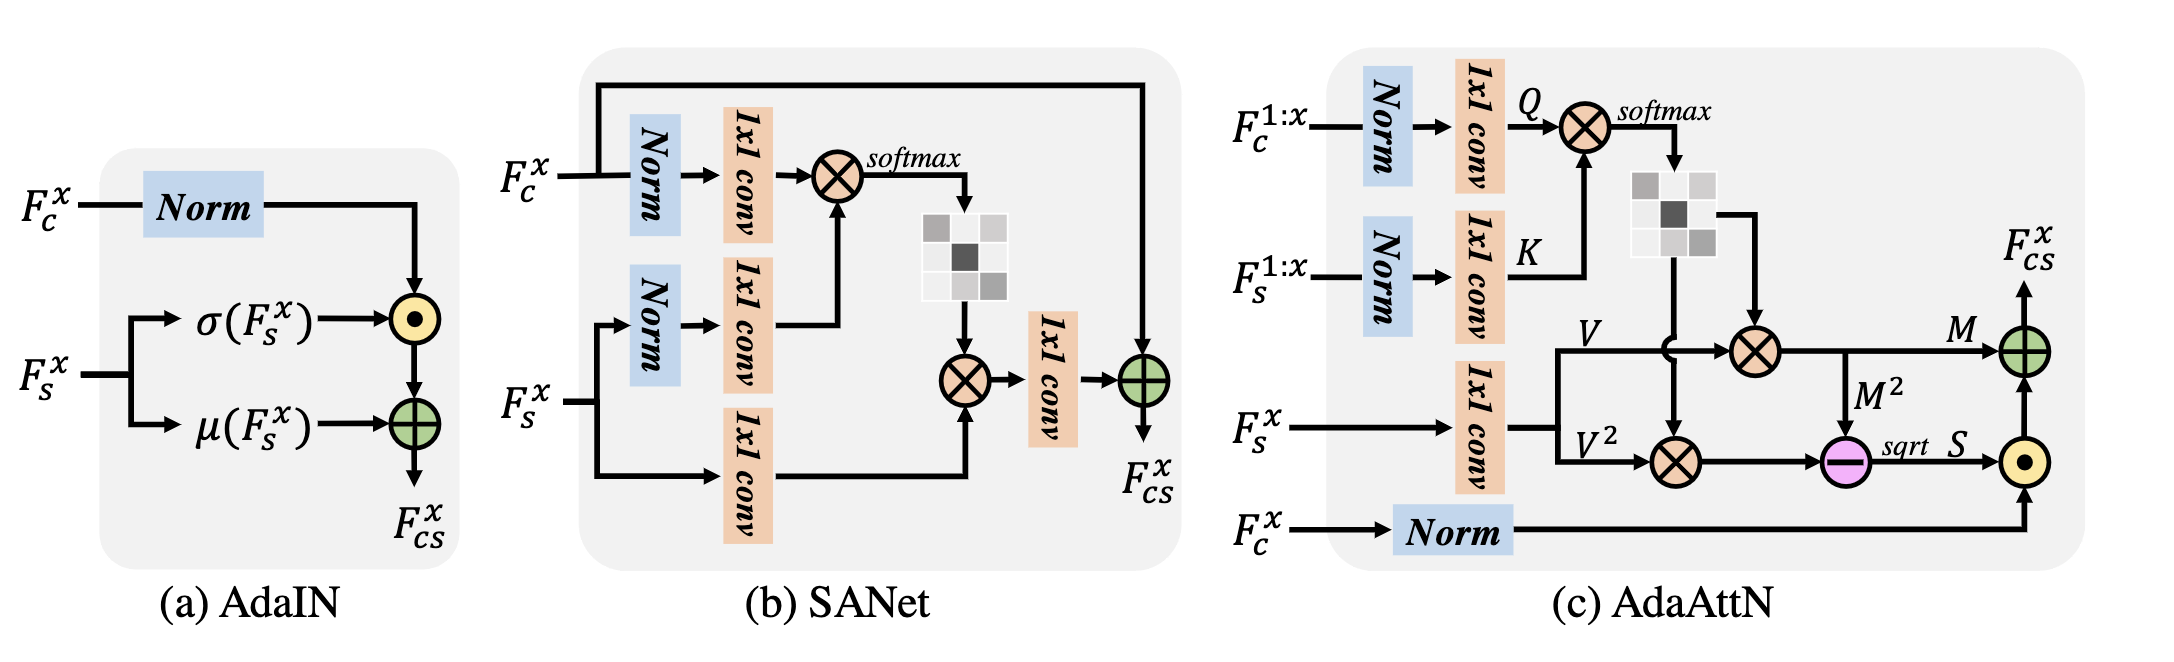
\includegraphics[width=\linewidth]{pics/diff_attn_p1}
    \caption{\label{fig:diff_adain_sanet_adaattn}三种方法在计算上的差别示意图}
\end{figure}

AdaAttN的总体流程如下:首先从浅层到深层计算包含内容和风格特征的注意力图,其中注意力机制被逐层计算用来衡量内容和风格特征之间的相似性。
随后基于注意力图计算风格特征的加权均值和标准差图。最后使用自适应归一化内容特征实现特征分布对齐。
针对SANet的问题,还有一些人对他做出了相应的优化。其中Chen等人~\cite{chen2021artistic}提出一种具有两种对比性损失的内部-外部风格转移方法。
它保留了风格注意力网络,并且利用单个风格图像的内部统计特征来确定风格化图像的颜色和纹理模式,
同时,还利用大规模风格数据集的外部信息来学习人类感知上的风格特征,
这使得风格化图像中的颜色分布和纹理模式更加合理和谐。
同时间,Deng等人~\cite{deng2022stytr2}提出了一种称为 StyTr2 的基于transformer的风格迁移模型。
该框架包括了一个新的感知内容位置编码(Content-Aware Positional Encoding,CAPE),其
中心思想是为图像风格迁移任务引入一种更加灵活和适应性的位置信息编码方式,
保证不同尺度的图像仍然有一致的空间关系。该模型认为风格图像不需要在编码期间严格保持位置关系,而内容图像需要,
故而该模型的风格图像编码器和内容图像编码器的唯一差别在于风格编码器没有应用CAPE。
经过训练以生成具有良好保留结构和输入内容图像细节的风格化结果。Ma等人~\cite{ma2023rast}提出了一种迭代的架构,
从图像修复的角度解决内容泄漏问题。可以通过多次的图像修复操作同时实现内容和风格信息的传输。
他们提出了两个新颖的损失函数--多修复损失和风格差异损失来确保更高的风格迁移质量。

\section{三维场景的风格迁移方法介绍}
近年来,随着科技的发展和人们收入的增加,人们对获取更优良的三维模型的需求也随之水涨船高。
三维的场景不仅可以提供更真实、更具体、更立体的展现形式,还可以使用户获得更加沉浸式的体验和感受。
三维风格迁移技术的核心目标是在保持三维场景结构和多视角一致性的同时,将指定图像的艺术风格自然地应用到三维模型上,
这项技术能够为艺术家和设计师提供强大的工具,使他们能够比较轻松地将特定的艺术风格应用到3D的场景环境中。
三维场景的风格迁移现有的研究基础较为丰富,从场景的表达方式上来看主要可以分为三类:基于显式三维数据表示的风格迁移方法、基于隐式神经辐射场
(Neural Radiance Field,NeRF)表示~\cite{mildenhall2021nerf}的风格迁移方法、基于三维高斯飞溅(3D Gaussian Splatting,3DGS)表示~\cite{kerbl20233d}的风格迁移方法。下面将逐一进行介绍。


\subsection{基于显式三维数据表示的风格迁移方法}
最早的方法是使用点云或者三角形网格来对真实场景进行建模。Huang等人~\cite{huang2021learning}使用VGG-19的编码器提取出模型的特征和风格图像的特征,
并且使用了一种新颖的聚合算法把特征融入,并且使用经过训练的解码器渲染生成新的风格化视图。Mu等人~\cite{mu20223d}的思路同Huang等人相似,
但是使用AdaAttN结合UNet网络进行单图的风格化新视角生成。尹等人~\cite{yin20213dstylenet}提出了3DSTYLENET,
它由两个主要网络组件即几何和纹理风格传输网络组成。首先在一组无纹理形状上预训练3D几何样式传递网络,
在图像数据集上预训练纹理样式传递网络。然后将几何和纹理进行联合优化。 
通过将形状和纹理样式从一个纹理网格转移到另一个纹理网格来创建 3D 网格的新颖几何和纹理变化。
但是这种方法的性能受到几何重建方法本身的质量的限制。随着后来新的高效的几何重建方法被提出,使用显式三维数据用于场景风格迁移的方法也逐渐在性能上不如新方法了。
\subsection{基于隐式神经辐射场表示的风格迁移方法}
相比而言,神经辐射场NeRF的提出很好地改善了几何重建领域的新视图合成质量差、表示方式不灵活、训练较慢等问题,具有重要的意义。
为了更有利于理解,本文拟先对该方法进行一个全面的介绍,然后再介绍基于NeRF表示的风格迁移方法研究现状。


%2.2.2.1
\paragraph{NeRF方法介绍}
NeRF方法由谷歌高级研究科学家Jon Barron在2020年首次提出,是一种基于深度学习的三维场景重建和渲染方法,它通过神经网络模拟场景的连续体积密度和颜色,
从而实现从二维图像数据中恢复出逼真的三维场景。NeRF的核心在于使用一系列从不同角度拍摄的图片来训练一个小型的神经网络,
该网络能够预测从任意视角观看场景时的体积密度和颜色。把物体看作一团可以自发光的粒子,这些粒子具有颜色C,密度σ两个属性。
使用现有的照片对体空间内粒子的密度和颜色进行预测,保存这些信息。在渲染其他视角时,使用这些信息(粒子的密度,颜色)进行推理,就能得到新视角下该场景的照片。NeRF的流程如\autoref{fig:nerf_show}所示:
\par 具体来说,NeRF要解决的问题就两个:
% \par 1. 如何通过现有的照片得到空间中密度与颜色的分布。
% \par 2. 如何利用这些数据,得到任意角度的照片。
\begin{enumerate}
    \item 如何通过现有的照片得到空间中密度与颜色的分布。
    \item 如何利用这些数据,得到任意角度的照片。
\end{enumerate}
\begin{figure}[htbp]
    \centering
    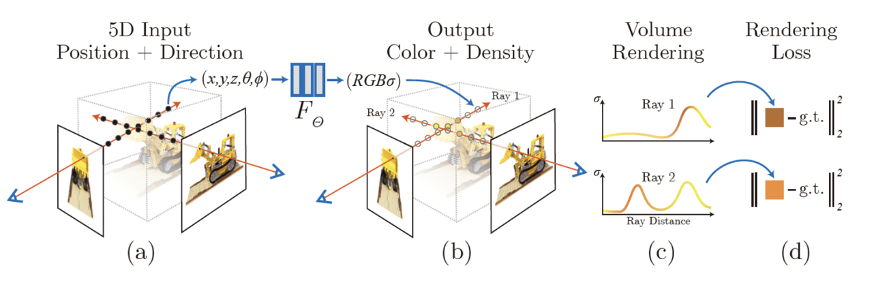
\includegraphics[width=\linewidth]{pics/nerf.png}
    \caption{\label{fig:nerf_show}NeRF方法的流程图}
\end{figure}



对于问题2,可以认为,从某一点看过去,这一点的颜色应该由达到这一点的光线上累积的颜色决定,想象每条光线路径上经过一个个小球到达最终像素上,
最终这些小球以自己的属性参与影响像素的颜色,这一计算可以用\autoref{equ:nerf_color_predict}表示:
% \begin{figure}[htbp]
%     \centering
%     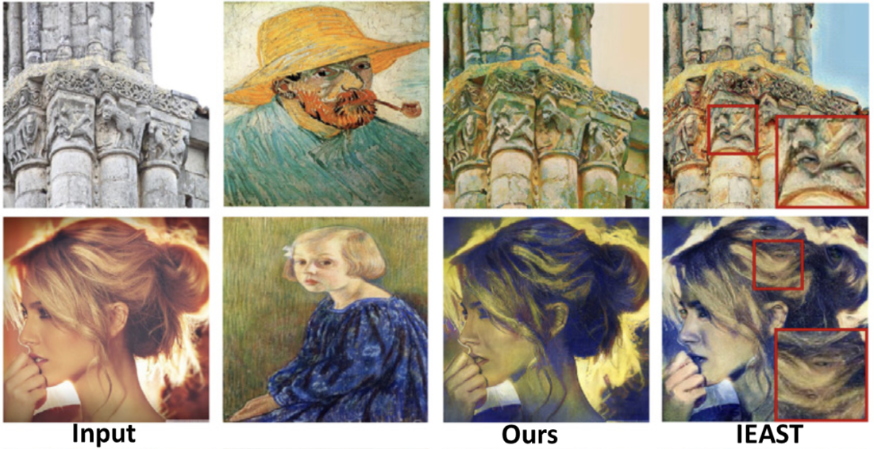
\includegraphics[width=\linewidth]{pics/pic_3.1.1}
%     \caption{\label{fig:pic_3.1.1}三种方法在计算上的差别示意图}
% \end{figure}
% aaa
% \begin{figure}[htbp]
%     \centering
%     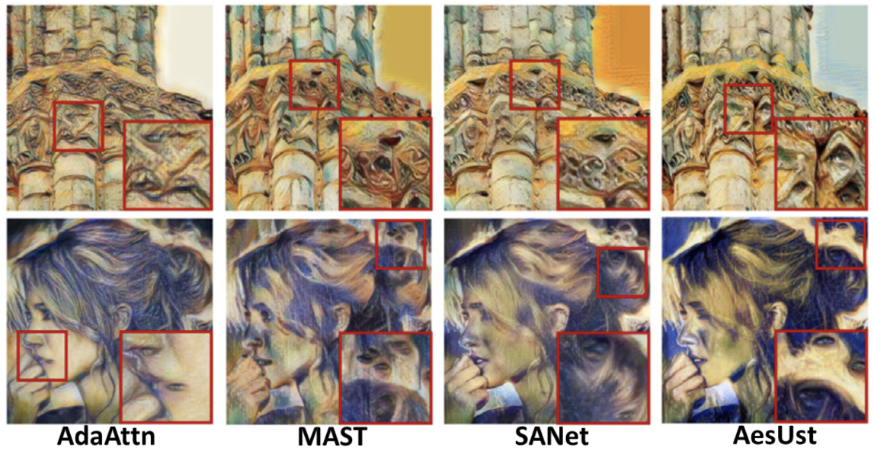
\includegraphics[width=\linewidth]{pics/pic_3.1.2}
%     \caption{\label{fig:pic_3.1.2}三种方法在计算上的差别示意图}
% \end{figure}

% t_n
% \autoref{equ:nerf_color_predict}
\begin{equation}
    \label{equ:nerf_color_predict}
    C^{p\text{redict}}(\mathbf{r})=\int_{t_n}^{t_f}T(t)\sigma(\mathbf{r}(t))\mathbf{c}(\mathbf{r}(t),\mathbf{d})dt
\end{equation}
其中$t_n$和$t_f$分别代表相机光线的近界和远界,$\mathbf{r}(t)=o+td$表示光线,$\sigma(t)$表示t处的密度,$\mathbf{c}(\mathbf{r}(t),\mathbf{d})$表示在$\mathbf{r}(t)$处以视角d看过去的颜色值,
$T(t)=\exp{(-\int_{t_n}^t\sigma(\mathbf{r}(s))ds)}$表示t处的不透明度。


\par 对于问题1,NeRF构建了一个神经网络$F_Θ$,其网络架构如\autoref{fig:nerf_net}所示:
\begin{figure}[htbp]
    \centering
    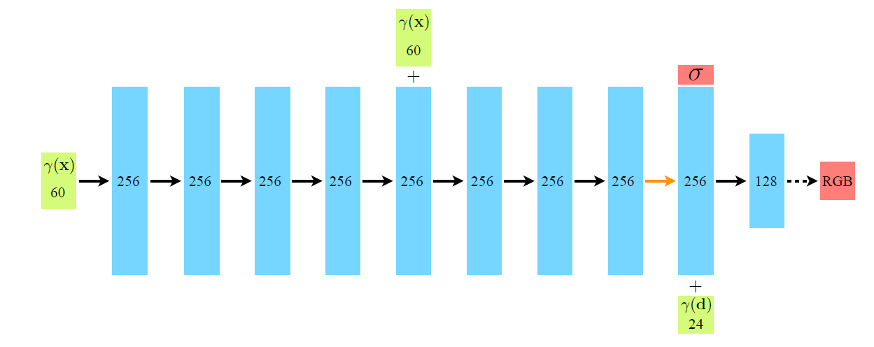
\includegraphics[width=\linewidth]{pics/nerf_net.png}
    \caption{\label{fig:nerf_net}NeRF方法的网络架构图}
\end{figure}




\par 输入为当前照片中,每个像素点看过来的角度,以及射线上采样点的坐标;输出为采样点上的颜色与密度。再利用上面的公式,计算得到预测的颜色 
% 再利用上面的公式,计算得到预测的颜色$\boldsymbol{C^{predict}}$,使用$\mathrm{MSE}(C^{ predict}-C)$作为约束进行训练。
\(\boldsymbol{C^{\text{predict}}}\)
使用 $\mathrm{MSE}(\boldsymbol{C}^{\text{predict}} - \boldsymbol{C})$ 作为约束进行训练。
但是,考虑到输入的信息粒度太粗,直接在神经网络中输入坐标与角度信息只有6维数据,网络可能无法提取到一些比较细微的差别,训练效果并不好。
比如对于同一点,不同角度看过去,这个角度值的变化可能并不大,但是看到的颜色差别很大。
\par 为了提取到高频信息、增强模型的学习和表示能力,需要对输入进行增强。NeRF采用了位置编码的方法,将3维空间位置坐标和角度信息使用正弦余弦函数进行编码,
增强后输入变为如\autoref{equ:nerf_pe}所示:

% \begin{equation}
%     \label{equ:nerf_pe}
%     (x,y,z)\to(x,y,z,sin(2^0,x),sin(2^0,y),sin(2^0,z),cos(2^0,x),cos(2^0,y),cos(2^0,z),...sin(2^{n-1},x),sin(2^{n-1},y),sin(2^{n-1},z),cos(2^{n-1},x),cos(2^{n-1},y),cos(2^{n-1},z)(\theta,\phi)\to(\theta,\phi,\sin{(2^0,\theta)},\sin{(2^0,\phi)},\cos{(2^0,\theta)},\cos{(2^0,\phi)},...sin(2^{m-1},\theta),sin(2^{m-1},\phi),cos(2^{n-1},\theta),cos(2^{n-1},\phi))
% \end{equation}
\begin{equation}
    \label{equ:nerf_pe}
    \begin{aligned}
        (x,y,z) \to & (x,y,z, \sin(2^0 x), \sin(2^0 y), \sin(2^0 z), \cos(2^0 x), \cos(2^0 y), \cos(2^0 z), \ldots, \\
                    & \sin(2^{n-1} x), \sin(2^{n-1} y), \sin(2^{n-1} z), \cos(2^{n-1} x), \cos(2^{n-1} y), \cos(2^{n-1} z)) \\
        (\theta,\phi) \to & (\theta,\phi, \sin(2^0 \theta), \sin(2^0 \phi), \cos(2^0 \theta), \cos(2^0 \phi), \ldots, \\
                          & \sin(2^{m-1} \theta), \sin(2^{m-1} \phi), \cos(2^{m-1} \theta), \cos(2^{m-1} \phi))
    \end{aligned}
\end{equation}
在实际操作中,一般取n=10,m=4,则最后输入MLP中的\(\gamma(\mathrm{x})\)和\(\gamma(\mathrm{d})\)维度可以得到分别是60和24。
	经过训练的NeRF模型,其中存储了一个场景的隐式信息,只要给定新视角的相机参数,可以很方便地用它进行新视角图片的渲染合成,而该方法也为三维场景的渲染提供了一个更强大的技术路线。


\paragraph{基于隐式神经辐射场表示的风格迁移方法综述}
较早把NeRF技术结合风格迁移并且取得较好效果的一个方法是Zhang等人~\cite{zhang2022arf}提出的风格化辐射场
(Artistic Radiance Field,ARF),它是一种新的可以将艺术特征从单个 2D 图像转移到完整的真实世界 3D 场景,
从而产生忠实于风格图像的艺术新颖视图渲染的方法。
该方法利用通过真实场景预训练的辐射场,并通过匹配从输入的2D风格图像中提取的特征将其转换为艺术辐射场,
从而通过渲染获得高质量的风格化新颖视图合成。它提出了两个贡献点。
首先,考虑到直接使用先前基于VGG的风格损失将包括风格图中诸如笔触、笔画等属性的丰富的视觉细节直接转移到3D场景是具有挑战性的,
因为由这种损失测量的风格信息通常基于全局统计特征、不一定能够以视图一致的方式很好地捕获局部细节这一问题,
作者提出了一个新的风格损失:最近邻特征匹配损失(Nearest Neighbor Feature Matching,NNFM)
以将复杂的高频视觉细节从2D风格图像转移到由辐射场参数化表示的3D场景,一致地跨多个视点。该损失函数的公式如\autoref{equ:nnfm}所示:
\begin{equation}
    \label{equ:nnfm}
    \ell_{\mathrm{nnfm}}(F_{\mathrm{render}},F_{\mathrm{style}})=\frac1N\sum_{i,j}minD(F_{\mathrm{render}}(i,j),F_{\mathrm{style}}(i^{\prime},j^{\prime}))
\end{equation}

其中$F_{render}$和$F_{Style}$分别是渲染后的图和风格图经过VGG-19编码器后得到的特征,
$F_{\mathrm{render}}(i,j)$代表特征图$F_{render}$在第(i,j)像素位置的特征向量,
N是$F_{render}$的像素数,$D(v_1,v_2)$计算两个向量$v_1$,$v_2$之间的余弦距离,其计算方式如\autoref{equ:cosine_distance}所示。
简而言之,对于$F_{render}$中的每个特征,采用最小化其到样式图像的VGG特征$F_{Style}$在VGG的特征空间中最近邻的余弦距离。
\begin{equation}
    \label{equ:cosine_distance}
    D(v_1,v_2)=1-v_1^Tv_2/\sqrt{v_1^Tv_1v_2^Tv_2}
\end{equation}


计算NNFM损失或者VGG特征损失的时候必须使用全分辨率图像,而不是图像的分块,而NeRF体渲染全分辨率图像的时候消耗大量内存。
为了解决这一问题,Zhang等人还提出了一个叫做“延迟反向传播”的方法,该方法通过以补丁方式累积缓存的梯度,
使场景参数能够以一个内存高效的方式在全分辨率图像上计算损失。为了追求更快的风格化速度,
Li等人~\cite{li2023instant}提出了快速神经辐射场风格化(Instant Neural Radiance Fields Stylization),
他们的方法使用InstantNGP中~\cite{muller2022instant}提出的多分辨率哈希编码。首先,他们将InstantNGP中的位置编码器分为两部分:
内容和样式。使用位置编码器,该网络可以在不到 10 分钟的时间内训练两个场景。
在对正常场景合成进行训练后,他们以内容和样式体素网格特征作为参考,在新视图合成的位置编码特征上执行AdaIN。
调整后的结果用于颜色预测,未调整的结果用于密度预测。该方法在保持相似的风格化质量的基础上实现了很大的速度提升。

\par 与Zhang等人同时期, Chiang等人~\cite{chiang2022stylizing}也提出了一种很新颖的保证风格化多视图一致性的方法。
他们使用超网络接受风格特征向量,并且据此输出该场景的NeRF模型的颜色MLP的参数。训练的时候首先训练NeRF模型的几何特性,
再对多个视角、多个风格分别最小化风格和内容损失以训练超网络习得风格的解码能力。
最终获得一个可以进行零样本场景风格迁移的网络。但是上述方法都无法捕捉较为局部的笔触风格信息。

\par Chen等人~\cite{chen2023testnerf}则考虑根据文本提示词来风格化场景并生成具有一致性的任意新视图。这是一个很有想法的尝试。
为了解决这个问题,他们首次设计了一个高效的文本驱动模型用于 3D 风格迁移,名为 TeSTNeRF。
通过跨模态学习对文本进行风格化:他们保留了Chiang等人~\cite{chiang2022stylizing}的超网络控制思路,
并利用高级文本编码器~\cite{radford2021learning}嵌入文本以控制 3D 风格迁移并在潜在空间中对齐输入文本并输出风格化图像。
此外,为了获得更好的视觉效果,他们引入了风格监督、从风格图像中学习特征统计并利用 2D 风格化结果来纠正突然的颜色溢出,
取得了较好的效果。但是文本相对于图像,其对于风格的描述能力有限,这也导致了在有的场景上风格化结果表现力不足等问题。

\par Chen等~\cite{chen2024upst}受到Chiang等人~\cite{chiang2022stylizing}的启发,也采用了超网络和超网络层学习风格潜向量的思想设计了UPST-NeRF,
但是他们没有直接修改隐式辐射场中存储的颜色信息,而是在查询阶段的MLP中对颜色进行修改,可以视为是一种“增量”的思想,
也可以看作是一个颜色解码器,对后面的方法影响深远。此外,为了更好地服务于真实感图像的风格化,
他们训练了一个 2D 逼真图像的风格迁移网络来处理不同视图下的真值 RGB 以获得目标,
在训练的时候对于每个视角每个风格都应用该网络获取风格化结果并用其来约束预测的颜色值。
但是他们这些方法都不能做到零样本迁移的同时还能保持较高的风格化质量。
为此,Liu等人~\cite{liu2023stylerf}提出了StyleRF,通过在辐射场的特征空间中执行风格迁移来尝试解决风格化的高精度重建、
高质量风格迁移、零样本快速迁移三方困境问题。具体来说,作者设计了采样不变的内容转换和延迟样式转换
(Sampling-Invariant Content Transformation 和Deferred Style Transformation),
前者通过严谨的数学论证消除对采样点批次的整体统计特征的依赖来确保多视图的一致性,
而后者通过将样式转换推迟到 2D 特征图上,大大提高了风格化效率。这个算法实现了很好的风格迁移效果和效率,
但是随着三维高斯飞溅方法的提出和应用,性能和效果逐渐被超越。下文将详细阐述3DGS方法和基于其的场景风格迁移方法概述。


\subsection{基于三维高斯飞溅表示的风格迁移方法}
三维高斯飞溅(3D Gaussian Splatting,3DGS)方法由Kerbl等人~\cite{kerbl20233d}在2023年提出,是多视角重建方面的突破性工作。它的特点在于使用3D高斯分布来表示场景,并且设计了一个创新的流水线,保持重建的高质量的情况下还能接入传统光栅化流水线,优化速度也快(能够以较少的训练时间,实现SOTA级别的NeRF的实时渲染效果,且可以以 1080p 分辨率进行高质量的实时(≥ 30 fps)新视图合成)。下面对该方法进行详细的介绍。
\paragraph{3DGS方法介绍}
神经辐射场方法彻底改变了用多张照片或视频捕捉的场景的可视化合成。然而,实现高质量的可视化仍然需要昂贵且训练和渲染速度缓慢的神经网络。
下面本段将对一种新颖的解决方案:3D 高斯飞溅技术进行一个简述。高斯飞溅是一种在90年代科学领域创建的渲染技术。
不过,它最近在去年 8 月的 SIGGRAPH 2023上展示的实时场景可视化应用,让它再次流行起来。
该技术和NeRF的区别大体上可以叙述为:对于场景表示,NeRF采用隐式辐射场表示,并且通过MLP查询得到某一位置的属性,而3DGS采用显式的高斯球进行表达,直接存储其特征属性;
对于渲染,NeRF是非常典型的backward mapping过程,即计算出每个像素点受到每个体素影响的方式来生成最终图像,对每个像素,投射出一条光线,并累积其路径上的颜色和不透明度。
而3DGS是forward mapping的过程,将每个体素视作一个模糊的球,投影到屏幕上。在溅射过程中,计算出每个体素如何影响每个像素点。
3DGS的优势在于:3D高斯表示允许优化最先进的视觉质量和竞争性训练时间,而基于分片的飞溅解决方案确保了渲染的高速度和高分辨率。
每个高斯球包括的属性有位置(平均值μ):存储了位置(XYZ)的空间坐标,协方差矩阵($\Sigma$):表征高斯球的旋转和缩放特性,不透明度($\alpha$):
代表每个高斯球的不透明程度,球谐 (SH) 系数:存储了每个高斯球的颜色特征。采用SH系数这样的各向异性属性可以允许非常灵活的优化机制。
该方法高效率的关键在于作者提出了一个基于分片的快速光栅化(tile-based rasterizer),它允许以$\alpha$-blending方式混合各向异性的溅射。
该快速光栅化器还包括实现了一个快速的反向传递,允许对任意数量的混合高斯进行有效的反向传播。本文提供的方法流程如\autoref{fig:3dgspipline}所示:

\begin{figure}[htbp]
    \centering
    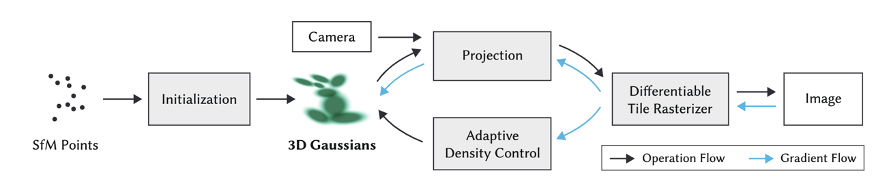
\includegraphics[width=\linewidth]{pics/3dgspipeline.png}
    \caption{\label{fig:3dgspipline}3DGS方法的管线图}
\end{figure}

具体来说,本文提出的方法优化从稀疏的SfM点云开始,并创建一组3D高斯,其将几何形状建模为一组不需要法线的3D高斯曲线。
提出的高斯分布由一个完整的三维协方差矩阵\(\Sigma=RSS^TR^T\)定义在世界空间中,$R$和$S$分别是旋转矩阵和缩放矩阵参数,以平均值μ为中心。其可以表达如\autoref{equ:3dgs_equ_main}所示:
% \autoref{equ:nerf_color_predict}
\begin{equation}
    \label{equ:3dgs_equ_main}
    G\left(x;\mu,\Sigma\right)=\frac1{\sqrt{(2\pi)^k\mid\Sigma\mid}}\exp\left(-\frac12(x-\mu)^T\Sigma^{-1}(x-\mu)\right)
\end{equation}
\par 随后,在渲染阶段,采用把3D高斯投影到2D平面上的方式,并使用提出的快速的基于分片的渲染器对此投影后的结果进行渲染。该渲染器使用了高度优化的光栅化管线和高性能的CUDA自定义内核,实现了快速的整体渲染和快速排序的目标,它有着极快的渲染速度和较小的额外内存消耗,可以对各种场景进行实时渲染。
\par 由于这一方法是从SfM初始化的,其高斯球的数量和密度必然不够精确。因此作者还提出了高斯函数的自适应性控制,简单来说,对于处于重建不足区域的小高斯函数,需要覆盖必须创建的新几何区域,因此采用克隆高斯球并且向位置梯度方向移动它的方法。对于高方差区域中的大高斯分布,它需要被分割成两个小高斯分布,并且把它们的尺寸都统一缩小一定值然后参与新一轮次的优化。
\paragraph{基于3DGS表示的风格迁移方法综述}
在3DGS方法的基础上,结合风格迁移技术,众多研究者加以研究和探索,开发出了一些很有效果的场景风格迁移算法。首先Chen等人~\cite{chen2024gaussianeditor}提出了GaussianEditor,是一个基于3DGS表示的快速可控三维可编辑场景的工作,它主要是用于场景编辑,但也可以用于风格迁移任务。它引入了高斯语义跟踪,从而实现更详细和有效的对象编辑控制。同时它还提出了分层的高斯飞溅(HGS),这是一种新的GS表示,根据高斯点的致密化轮次进行分类并对它们进行逐步收缩的限制,这能够在高度随机的生成引导下更稳定地收敛到细化的结果。同时,它设计了一种用于高斯飞溅的3D修复算法,该算法可以快速去除和添加对象,更方便执行可控的场景编辑工作。但是本工作主要依靠预训练的多模态大语言所学到的丰富先验知识引导风格化操作,相比于使用蕴含丰富细节、内容信息的图像引导的风格迁移工作稍显不足,但是这是一个很好的探索。

\par 第一个真正意义上使用3DGS的表示用于图片引导的场景风格迁移工作是Sahara等人~\cite{saroha2024gaussian}提出的GSS,他们提出使用InstantNGP中提出的多分辨率哈希编码来对已经初始化完成的高斯点集进行升维表示,多分辨率哈希编码在每一层都是独立的,并且高度适应所需的最佳分辨率。因此,它在训练期间实现了更快的收敛,不会阻碍推理速度,并促进更高级别的细节,这有利于使用 3DGS 表示的风格化任务。随后,GSS提出了一个3D颜色模块,把每个风格化图的潜向量和每个高斯点的查询结果拼在一起并且使用一个MLP进行计算得到高斯点风格化后的颜色。该方法能够准确地生成场景中每个 3D 高斯的风格化颜色,并且以很高的速度渲染生成新的视角,这得益于3DGS本身相对于NeRF方法的速度优势。但是由于该方法仅使用AdaIN来做风格化监督,其生成的场景依然不太考虑风格图像的笔触、线条特征等艺术问题。

\par Zhang等人~\cite{zhang2024stylizedgs}提出了StylizedGS,它可以支持可调整的控制因子,以改变控制强度,并提出了一种GS过滤器来消除重建中的会影响风格化效果的漂浮物,然后引入基于最近邻的样式损失NNFM,通过微调3DGS的几何和颜色参数来实现风格化,同时提出了一种具有其他正则化的深度保存损失,以防止几何内容被大幅度修改。本文的高斯点风格化操作通过颜色的直方图匹配算法实现。

\par Yu等人~\cite{yu2024instantstylegaussian}提出InstantStyleGaussian,该方法主要依赖于图像提示,并利用文本辅助生成训练数据集。总的来说该方法使用图像的条件扩散模型用于迭代更新训练数据集图像,然后对重建的场景模型进行微调以匹配参考编辑的图像样式,最终生成符合艺术风格的场景,同时保持3D一致性。该方法实现了具有更高质量风格化的3D 场景风格迁移,提高了速度和性能。但是该方法的效果依赖于图像的扩散模型的性能。相信随着更强大的图像处理扩散模型的出现,该方法更好的风格化效果将会可以期待。

\par Liu等人~\cite{liu2024stylegaussian}提出了StyleGaussian,它允许以每秒10帧的速度将任何图像的样式即时地迁移到3D场景中。利用3D高斯飞溅(3DGS),StyleGaussian在不影响其实时渲染能力和多视图一致性的情况下实现了样式转移。它把三维场景风格迁移的通用流程总结为:特征嵌入、风格迁移和解码渲染。最初,2D 图像的VGG场景特征被嵌入到重建的3D高斯中。接下来,根据参考风格图像对嵌入的特征进行变换。最后,将转换后的特征解码为风格化的 RGB。StyleGaussian 有两种新颖的设计。第一个是一种有效的特征渲染策略,它显著减少了内存消耗。它首先渲染低维特征,然后将它们映射到高维特征,同时嵌入VGG 特征,这样解决了 3DGS 不能够渲染高维内存密集型特征的问题。第二个是基于K最近邻的 3D CNN解码器。这种解码器直接在3D空间中工作,可以很好地保持多视图一致性并且不影响3D高斯渲染的速度。

\par \(\text{Kovács}\)等人~\cite{kovacs2024g}提出了G-style,该文章认为现有的基于3DGS的场景迁移方法不会改变表示场景的高斯的位置和形状,这将会导致场景的某些区域的分辨率较低。除了上述问题外,所有 3D 风格迁移方法只关注从风格图像中转移高频模式,例如笔触或颜色统计。然而,图像风格的概念更加微妙,并且与图像有很大不同。G-style首先在预处理步骤中删除了具有大投影区域或高度拉长形状的不良高斯点,并且限制只使用球谐函数的第0阶以保证只有漫反射属性。为了确保最终的风格化3D场景与原始风格图像之间的颜色分布相似,在算法开始时,将真实图像与风格图像的颜色的均值和协方差矩阵进行匹配。随后作者结合了几个精心设计的损失来保留图像中风格的不同比例,同时保持原始场景内容的完整性尽可能高。为了更好的提高某些低分辨率部分的风格化质量,在风格化过程中通过跟踪风格化颜色的梯度来拆分在场景中需要额外的细节的高斯。为了克服高斯点数量过多这个问题,在风格化过程中,作者还添加了一个高斯点的微调步骤,根据它们的风格属性的梯度周期性地拆分高斯函数。

\par 为了获得更高质量的指定区域风格化,Jain等人~\cite{jain2024stylesplat}提出了StyleSplat,这是一种轻量级的方法,用于从参考样式图像中对由3D高斯表示的场景中的部分3D对象进行风格化。该方法首先使用 3D 高斯溅射学习场景的逼真表示,同时使用语义分割大模型SAM~\cite{kirillov2023segment}联合分割单个 3D 对象。随后使用最近邻特征匹配损失NNFM来微调所选对象的高斯属性,将它们的球谐系数与样式图像对齐,以确保一致性和视觉吸引力。StyleSplat允许场景中多个对象的快速、可定制的样式转移和局部风格化,每个对象都有不同的样式。

\par 上述方法除了最后提出的几个同期工作以外,均可以在性能方面继续提升,以让风格化效果更加精致、支持更快的零样本风格迁移等。这正是本文的目标之一,相关细节将在本文第四章予以详细说明。

\section{对比学习技术}
由于本文所提出的方法需要使用到对比学习方法来学习从风格化到风格化的关联,故本文在此对这一技术进行一个介绍。对比学习由三个关键要素组成:查询、正例和负样本。对比学习背后的基本思想是鼓励相似的实例在学习的嵌入空间中被映射得更近,同时将不相似的实例推得更远。通过将学习视为一项辨别任务,对比学习允许模型捕获数据中的相关特征和相似性。对比学习由以下几个步骤构成:数据增强、特征提取、投影网络、对比学习的目标、损失函数、训练和优化、评估。
\par 数据增强:对比学习方法的初始阶段是数据增强。数据增强的主要目标是增强数据的异构性,从而将模型引入相同实例的多个视角。此步骤涉及应用各种转换技术,包括裁剪、翻转、旋转和额外扰动来生成一系列数据表示。实例的多样化有助于确保对比学习模型能够吸收相关信息,而不管输入数据中存在的变化。
\par 特征提取:数据增强之后,对比学习过程使用编码器网络将增强的实例转置到潜在表征空间来发挥作用。这种能力对于模型区分相似实例和不相似实例至关重要。编码器网络的架构通常由先进的神经网络模型构成,例如用于图像数据集的卷积神经网络 (CNN) 或用于序列数据的循环神经网络 (RNN)等。
\par 投影网络:投影网络负责将编码器网络的输出映射到为更紧凑、更低维的空间。此阶段对于增强模型的辨别能力至关重要。通过将表示转移到低维框架中,投影网络有效地减轻了数据复杂性和冗余度。这种减少对于在数据集内实现相似实例和不相似实例之间的更明显区分起着关键作用。
\par 对比学习的目标:将增强实例编码并投影到嵌入空间后,即可系统地应用对比学习目标。
该目标的设计有两个重点:首先,最大化来自同一样本的实例之间的一致性;其次,最小化来自不同样本的实例之间的一致性。
这种策略方法激励模型在表征空间中拉近具有相似性的实例,同时疏远不相似的实例。实例之间的相似度量化通常采用距离度量,其中欧几里得距离或余弦相似度是常用的度量。
损失函数:对比学习任务有许多不同的损失函数,每个损失函数的设计目的都是为了促进获取能够巧妙地概括数据集内基本相似性和差异性的表示。
可用于风格迁移领域比较著名的损失函数有:ContraGAN~\cite{kang2020contragan}提出了一个条件对比学习损失函数(Conditional Contrastive Loss,2C loss)
来学习样本到类和样本到样本的关系。OpenAI~\cite{radford2021learning}提出的对比语言-图像预训练损失(CLIP Loss)构建了语言和图像之间的有效关系。
CLIP通过对比学习的方式,将图像和文本嵌入到同一个语义空间中,使得模型能够理解图像和文本之间的语义关系。
CLIP模型的核心思想是通过最大化图像表示与其相应文本描述之间的一致性,来预训练一个能够同时理解图像和文本的模型。
对比学习是CLIP模型的核心,它通过比较正样本(匹配的图像-文本对,即图中对角线上N个匹配的图像-文本对)和负样本(不匹配的对,即$N^2-N$个没有匹配的图像-文本对)来训练模型。
这种学习策略使得模型能够学习到图像和文本之间的复杂关系,而不仅仅是简单的特征对应。CLIP的对比学习框架提高了模型对视觉和语言数据的泛化能力。
这使得我们可以把CLIP模型的思想运用到图像的风格迁移中来。\autoref{fig:clip_intro}是CLIP的说明示意图。CLIP 可以生成良好的视觉表示,
可以非常轻松地迁移到许多计算机视觉领域的基准数据集,从而实现与有监督的基线方法相媲美的结果。
\begin{figure}[htbp]
    \centering
    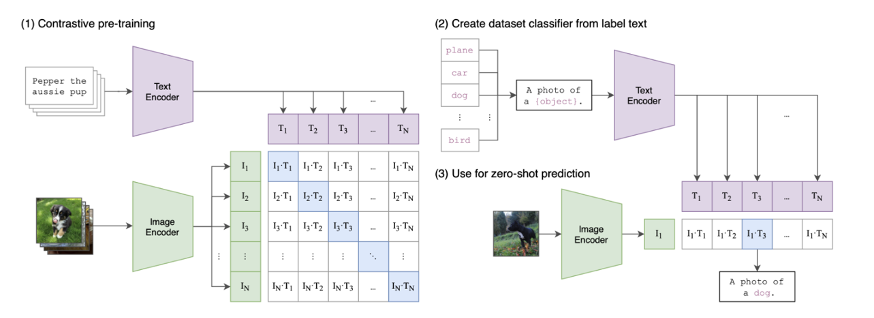
\includegraphics[width=\linewidth]{pics/clip_introduction.png}
    \caption{\label{fig:clip_intro}3DGS方法的管线图}
\end{figure}
\par 训练和优化:在定义损失函数后,模型会使用大量数据集(主要是未标记的数据集)进行训练。这个训练过程是迭代的,涉及不断更新模型的参数以最小化损失函数。这种迭代优化逐步细化所学习到的表示,从而增强模型有效区分和区分相似和不相似实例的能力。
\par 在风格迁移的领域,Chen等人~\cite{chen2021artistic}首先基于预训练的VGG模型构建正样本和负样本,以学习风格化到风格化的关系。Zhang等人~\cite{zhang2022domain}全面介绍了使用视觉特征进行风格表示的对比学习,以表示任意风格转移的风格。Wu等人~\cite{wu2022ccpl}设计了一种通用的对比相干保持损失来学习局部斑块。
CLIPstyler~\cite{kwon2022clipstyler}引入了一个文本引导的合成模型,可以根据特定的文本传输图像的风格。这些方法都在一定程度上保留了内容图像的内容并增强了风格化图像的风格,给本文提供了思路上的启发。

\section{评价指标}
风格迁移是一类试图合成艺术风格化的视觉媒介的方法。为了评估风格化的性能结果,使用了多种评估方法和指标,包括统计参与者主观判断的人类视觉效果评估,
以及客观评估算法性能不同方面的大量定量计算指标。然而,对于能够保证结果可靠性的最合适和最有效的评价手段,
由于艺术风格这一概念的模糊性,和高度主观性,目前在客观指标的选用上还没有达成共识。
现用的计算指标试图量化内容留存率、风格相似性和整体效率这些因素。尽管有大量的评估方法,
但评估过程在NST算法之间是不同的。根据媒介的不同,也取决于一种方法旨在实现的特定进步或贡献,
每种风格转移方法都采用不同的评估程序。评估NST方法的产出所涉及的主观性,每种方法的特定意图和目标,
以及每种方法试图解决风格化问题的角度,使评估成为一项复杂而苛刻的活动。经过认真地调研,
决定本文的评估决定从主观和客观两个角度进行评估。其中主观角度采用欺骗分数(Deception Score)。
欺骗分数表示用户把生成的风格化鉴定为真实艺术图像的比率。
更高的分数意味着该风格化图像被更高比例人鉴定为真实风格化作品。
客观角度采用内容保真度(Content Fidelity,CF), 全局影响分数(Global Effects ,GE)和本地图样分数(Local Patterns ,LP)~\cite{wang2021evaluate}指标,
保证指标覆盖了感知和风格化表现这两个方面,用于二维图像风格迁移的效果评估,采用长短期一致性用于三维图像风格迁移的效果评估,
并且采用ArtFID~\cite{wright2022artfid}和结构相似性(Structural Similarity,SSIM)~\cite{wang2004image}等指标用于场景风格化后渲染得到的2D风格化图像的质量评估,
采用短程一致性和长程一致性(Short-range Consistency和Long-range Consistency)~\cite{lai2018learning}用于3D场景的风格化一致性质量评估,并在下文对这些指标进行详细解释说明。
\par CF是用来衡量在多个尺度上对内容特征的忠实度。它基于这样一个看法:令人印象深刻的风格转移结果应该携带足够的风格特征,同时保留明显感知的内容结构。其公式如\autoref{equ:equ_cal_cf}所示:

\begin{equation}
    \label{equ:equ_cal_cf}
    CF(\vec{x},\vec{c})=\frac1N\sum_{l=1}^N\frac{f_l(\vec{x})\cdot f_l(\vec{c})}{\parallel f_l(\vec{x})\parallel\cdot\parallel f_l(\vec{c})\parallel}
\end{equation}
其中$\vec{c}$和$\vec{x}$分别是内容图像和风格化结果,\(f_l(\cdot)\)表示从第l层提取的特征激活。N是不同层的数量。
\par GE用来衡量全局相似性。在将转移的风格与风格图像进行比较时,人们经常首先欣赏全局效果。全局相似性将对人类视觉感知留下初步印象,
因此它是衡量风格化质量的重要因素。通过调查作者认为颜色和纹理更容易影响观察者的评估,因此全局效应 (GE) 因子应包括这两个方面,
即全局颜色 (GC) 和整体纹理 (HT)。对于GC的计算,直接比较颜色直方图的余弦相似度以利用RGB颜色空间中的颜色信息,其计算方式如\autoref{equ:equ_cal_gc}所示,对于HT的计算,
利用Gatys等人提出的~\cite{gatys2016image,gatys2017controlling}风格表示 (Gram 矩阵),这已被证明可以有效地表达图像的整体纹理。其计算方式如\autoref{equ:equ_cal_ht}所示:
\begin{equation}
    \label{equ:equ_cal_gc}
    GC(\vec{x},\vec{s})=\frac13\sum_{c=1}^3\frac{hist_c(\vec{x})\cdot hist_c(\vec{s})}{\parallel hist_c(\vec{x})\parallel\cdot\parallel hist_c(\vec{s})\parallel}
\end{equation}
其中$\vec{s}$是风格图像,\(hist_c(\cdot)\)表示由通道$c$得到的颜色直方图向量。
\begin{equation}
    \label{equ:equ_cal_ht}
    HT(\vec{x},\vec{s})=\frac1N\sum_{l=1}^N\frac{G(f_l(\vec{x}))\cdot G(f_l(\vec{s}))}{\parallel G(f_l(\vec{x}))\parallel\cdot\parallel G(f_l(\vec{s}))\parallel}
\end{equation}
其中$G(⋅)$表示Gram矩阵。由于认为这两个因素都是同等重要的,因此最后通过计算二者平均值得到GE分数,如\autoref{equ:equ_cal_ge}所示:
\begin{equation}
    \label{equ:equ_cal_ge}
    GE(\vec{x},\vec{s})=\frac12(GC(\vec{x},\vec{s})+HT(\vec{x},\vec{s}))
\end{equation}
\par LP指标的灵感来源于:在大致感知全局效果后,人们会放大观察一些局部风格模式的相似性,
如笔触、精美图案、详细的纹理等。
因此,定义了一个局部模式(LP)因子来衡量这一方面的质量。
受到人类评估中考虑的元素的启发,该LP 因子由两部分组成,一是直接评估局部模式对应物的相似性,
二是比较检索到的模式类别的多样性。一个好的风格化结果应该类似于风格图像,不仅在相应的局部模式中,而且在检索到的模式类别的多样性上。首先用神经网络对神经特征
\(f_l(\vec{x})\)和\(f_l(\vec{s})\)提取一组3 × 3的块(patch),记为\(\{\Phi_i^l(\vec{x})\}_{i\in n_x}\)和\(\{\Phi_j^l(\vec{s})\}_{j\in n_s}\),
其中$n_x$和$n_s$分别是内容图像和风格图像的块数。对于每一个\(\Phi_i^l(\vec{x})\),我们根据以下归一化相关度确定最匹配的样式块\(\Phi_{CM(i)}^l(\vec{s})\),
如\autoref{equ:equ_cal_tmp_phi_cmi}所示:
\begin{equation}
    \label{equ:equ_cal_tmp_phi_cmi}
    \Phi_{CM(i)}^l(\vec{s}){:}=\arg\max_{j=1,...,n_s}\frac{\Phi_i^l(\vec{x})\cdot\Phi_j^l(\vec{s})}{\parallel\Phi_i^l(\vec{x})\parallel\cdot\parallel\Phi_j^l(\vec{s})\parallel}
\end{equation}
随后可以定义LP为$LP_1$和$LP_2$两部分,如\autoref{equ:equ_cal_lp1}和\autoref{equ:equ_cal_lp2}所示:
\begin{equation}
    \label{equ:equ_cal_lp1}
    LP_1(\vec{x},\vec{s})=\frac1Z\sum_{l=1}^N\sum_{i=1}^{n_x}\frac{\Phi_i^l(\vec{x})\cdot\Phi_{CM(i)}^l(\vec{s})}{\parallel\Phi_i^l(\vec{x})\parallel\cdot\parallel\Phi_{CM(i)}^l(\vec{s})\parallel}
\end{equation}
其中\(Z=N\times n_x\),这一部分测量了\(f_l(\vec{x})\)和\(f_l(\vec{s})\)所对应的局部图样的相似性。
另一部分直接通过比较不同的神经块的类数目来定义。
\begin{equation}
    \label{equ:equ_cal_lp2}
    LP_2(\vec{x},\vec{s})=\frac1N\sum_{l=1}^N\frac{t_{cm}^l}{t_s^l}
\end{equation}
其中$t_{cm}^{l}$和$t_{s}^{l}$分别代表
$\{\Phi_{CM(i)}^l(\vec{s})\}$和$\{\Phi_j^l(\vec{s})\}$
中不同块的数量。考虑到两者一致的重要程度,最终可以得到总的LP分数如\autoref{equ:equ_cal_lp_all}所示:
\begin{equation}
    \label{equ:equ_cal_lp_all}
    LP(\vec{x},\vec{s})=\frac12(LP_1(\vec{x},\vec{s})+LP_2(\vec{x},\vec{s}))
\end{equation}
\par SSIM~\cite{wang2004image}是一个经典的评估指标,它从三个方面综合评价图像质量:亮度相似性、对比度相似性、结构相似性。它的计算流程如\autoref{fig:img_ssim_cal}所示:

\begin{figure}[htbp]
    \centering
    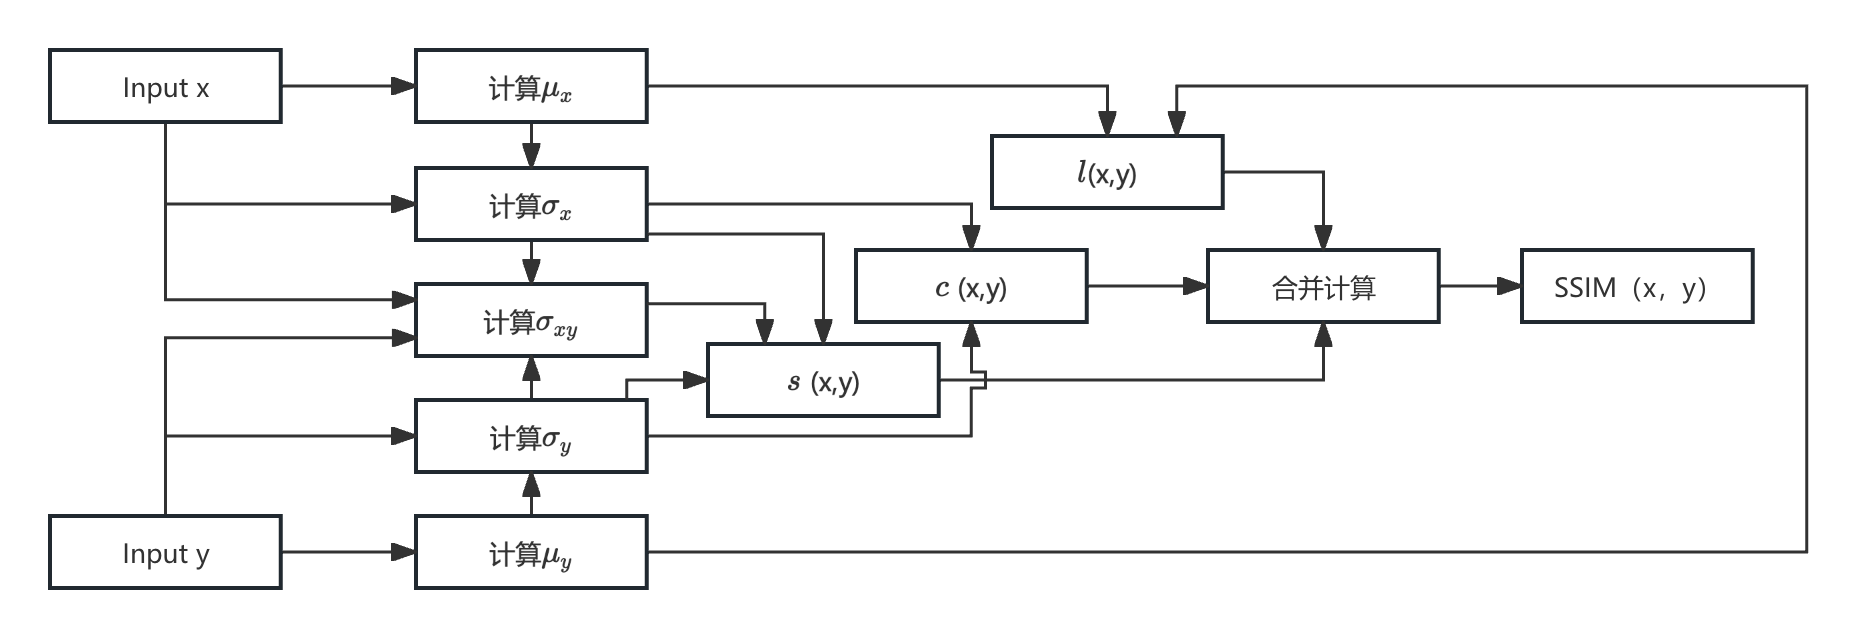
\includegraphics[width=\linewidth]{pics/ssim_cal.png}
    \caption{\label{fig:img_ssim_cal}3DGS方法的管线图}
\end{figure}
在该图中的亮度相似性的定义如\autoref{equ:equ_cal_ssim_lxy}所示:
\begin{equation}
    \label{equ:equ_cal_ssim_lxy}
    \mathrm{l(x,y)=\frac{2\mu_x\mu_y+C_1}{\mu_x^2+\mu_y^2+C_1}}
\end{equation}
其中\(\mu_\mathrm{x}=\frac{1}{\mathrm{N}}\sum_{\mathrm{i}=1}^\mathrm{N} \mathrm{x_i}, \mu_\mathrm{y}=\frac{1}{\mathrm{N}}\sum_{\mathrm{i}=1}^\mathrm{N} \mathrm{y_i}, \mathrm{C_1}\)
是一个防止分母为零的常数。对比度相似性的定义如\autoref{equ:equ_cal_ssim_cxy}所示:
\begin{equation}
    \label{equ:equ_cal_ssim_cxy}
    \mathrm{c}(\mathbf{x},\mathbf{y})=\frac{2\sigma_\mathrm{x}\sigma_\mathrm{y}+\mathrm{C}_2}{\sigma_\mathrm{x}^2+\sigma_\mathrm{y}^2+\mathrm{C}_2}
\end{equation}
其中,\(\sigma_{\mathrm{x}}=\left(\frac1{\mathrm{N}-1}\Sigma_{\mathrm{i}=1}^{\mathrm{N}}\left(\mathrm{x}_{\mathrm{i}}-\mu_{\mathrm{x}}\right)^{2}\right)^{\frac12},\sigma_{\mathrm{y}}=\left(\frac1{\mathrm{N}-1}\Sigma_{\mathrm{i}=1}^{\mathrm{N}}\left(\mathrm{y}_{\mathrm{i}}-\mu_{\mathrm{y}}\right)^{2}\right)^{\frac12},C_{2}\)
的作用和\(C_1\)相同。结构相似性的定义如\autoref{equ:equ_cal_ssim_sxy}所示:
\begin{equation}
    \label{equ:equ_cal_ssim_sxy}
    \mathrm{s(x,y)=\frac{\sigma_{xy}+C_3}{\sigma_x\sigma_y+C_3}}
\end{equation}
其中,\(C_3\)的作用和\(C_2、C_1\)相同,都是为了防止分母出现零,而\(\sigma_{\mathrm{xy}}\)是x和y的协方差,其可以按\autoref{equ:equ_cal_ssim_covxy}计算:
\begin{equation}
    \label{equ:equ_cal_ssim_covxy}
    \sigma_{\mathrm{xy}}=\frac1{\mathrm{N}-1}\sum_{\mathrm{i}=1}^{\mathrm{N}}(\mathrm{x_i}-\mu_\mathrm{x})(\mathrm{y_i}-\mu_\mathrm{y})
\end{equation}
有了上述三个公式后,\(\mathrm{SSIM}(\mathbf{x},\mathbf{y})\)可以按\autoref{equ:equ_cal_ssim}计算:
\begin{equation}
    \label{equ:equ_cal_ssim}
    \mathrm{SSIM}(\mathbf{x},\mathbf{y})=[\mathrm{l}(\mathbf{x},\mathbf{y})]^\alpha\cdot[\mathrm{c}(\mathbf{x},\mathbf{y})]^\beta\cdot[\mathrm{s}(\mathbf{x},\mathbf{y})]^\gamma 
\end{equation}
其中的\(\alpha,\beta,\gamma \)分别用于调控三个部分的权重。特别地,当\(\alpha{=}\beta{=}\gamma{=}1\text{,且}C_3=C_2/2\)的时候,
SSIM可以简化为如\autoref{equ:equ_cal_ssim_simplified}的形式,这也是计算SSIM常用的形式。需要指出,SSIM计算实在每个图像局部块上,最后需要pooling来得出整幅图像分数,
论文采用的是简单的average pooling方式,即求平均值。
\begin{equation}
    \label{equ:equ_cal_ssim_simplified}
    \mathrm{SSIM}(\mathbf{x},\mathbf{y})=\frac{(2\mu_\mathrm{x}\mu_\mathrm{y}+\mathrm{C}_1)(2\sigma_\mathrm{xy}+\mathrm{C}_2)}{(\mu_\mathrm{x}^2+\mu_\mathrm{y}^2+\mathrm{C}_1)(\sigma_\mathrm{x}^2+\sigma_\mathrm{y}^2+\mathrm{C}_2)}
\end{equation}

% 我们可以用includegraphics来插入现有的jpg等格式的图片,
% 如\autoref{fig:zju-logo}所示。

% \begin{figure}[htbp]
%     \centering
%     
\includegraphics[width=.3\linewidth]{logo/zju}
%     \caption{\label{fig:zju-logo}浙江大学LOGO}
% \end{figure}





% \par 如\autoref{tab:sample}所示,这是一张自动调节列宽的表格。

% \begin{table}[htbp]
%     \caption{\label{tab:sample}自动调节列宽的表格}
%     \begin{tabularx}{\linewidth}{c|X<{\centering}}
%         \hline
%         第一列 & 第二列 \\ \hline
%         xxx & xxx \\ \hline
%         xxx & xxx \\ \hline
%         xxx & xxx \\ \hline
%     \end{tabularx}
% \end{table}



\chapter{另一章}


\begin{figure}[htbp]
    \centering
    \includegraphics[width=.3\linewidth]{example-image-a}
    \caption{\label{fig:fig-placeholder}图片占位符}
\end{figure}

\chapter{再一章}

\par 如\autoref{alg:sample},这是一个算法

\begin{algorithm}[H]
    \begin{algorithmic} % enter the algorithmic environment
        \REQUIRE $n \geq 0 \vee x \neq 0$
        \ENSURE $y = x^n$
        \STATE $y \Leftarrow 1$
        \IF{$n < 0$}
            \STATE $X \Leftarrow 1 / x$
            \STATE $N \Leftarrow -n$
        \ELSE
            \STATE $X \Leftarrow x$
            \STATE $N \Leftarrow n$
        \ENDIF
        \WHILE{$N \neq 0$}
            \IF{$N$ is even}
                \STATE $X \Leftarrow X \times X$
                \STATE $N \Leftarrow N / 2$
            \ELSE[$N$ is odd]
                \STATE $y \Leftarrow y \times X$
                \STATE $N \Leftarrow N - 1$
            \ENDIF
        \ENDWHILE
    \end{algorithmic}
    \caption{\label{alg:sample}算法样例}
\end{algorithm}